\documentclass[10pt]{article}

\usepackage[T1]{fontenc}
\usepackage[utf8]{inputenc}
%\usepackage{beton}
%\usepackage{ccfonts}
%\usepackage{concrete}
\usepackage{concmath}
\usepackage{eulervm}
\usepackage{amsmath,amsthm,amssymb}
\usepackage{mathtools}
\usepackage{multicol}
\usepackage{marginnote}
\usepackage{pgfplots}
\usepackage{float}
\usepackage{hyperref}
\usepackage{bbm}
\usepackage{booktabs}
\usepackage{xcolor-solarized}
\usepackage{xcolor}
\usepackage{accents}
\pgfplotsset{compat=1.5}

\usepackage{listings}
\usepackage{xcolor}
\definecolor{codegreen}{rgb}{0,0.6,0}
\definecolor{codegray}{rgb}{0.5,0.5,0.5}
\definecolor{codepurple}{rgb}{0.58,0,0.82}
\definecolor{backcolour}{rgb}{0.95,0.95,0.92}
\lstdefinestyle{mystyle}{
    backgroundcolor=\color{backcolour},   
    commentstyle=\color{codegreen},
    keywordstyle=\color{magenta},
    numberstyle=\tiny\color{codegray},
    stringstyle=\color{codepurple},
    basicstyle=\ttfamily\footnotesize,
    breakatwhitespace=false,         
    breaklines=true,                 
    captionpos=b,                    
    keepspaces=true,                 
    numbers=left,                    
    numbersep=5pt,                  
    showspaces=false,                
    showstringspaces=false,
    showtabs=false,                  
    tabsize=2
}

\lstset{language=Python, style=mystyle}

\usepackage{mathtools}

\usepackage{wasysym}
\usepackage[margin=1.5in]{geometry} 
\usepackage{enumerate}
\index{\usepackage}\usepackage{multicol}

\newcommand{\N}{\mathbf{N}}
\newcommand{\Z}{\mathbb{Z}}

\newcommand{\R}{\mathbf{R}}
\newcommand{\C}{\mathbf{C}}
\newcommand{\Pbb}{\mathbb{P}}
\newcommand{\Fcal}{\mathcal{F}}
\newcommand{\Lcal}{\mathcal{L}}
\newcommand{\Acal}{\mathcal{A}}
\newcommand{\Ecal}{\mathcal{E}}
\newcommand{\Ebb}{\mathbb{E}}
\newcommand{\Qbb}{\mathbb{Q}}


\renewcommand{\mathbf}{\mathbold}

\newenvironment{theorem}[2][Theorem]{\begin{trivlist}
  \item[\hskip \labelsep {\bfseries #1}\hskip \labelsep {\bfseries #2.}]}{\end{trivlist}}
\newenvironment{lemma}[2][Lemma]{\begin{trivlist}
  \item[\hskip \labelsep {\bfseries #1}\hskip \labelsep {\bfseries #2.}]}{\end{trivlist}}
\newenvironment{exercise}[2][Exercise]{\begin{trivlist}
  \item[\hskip \labelsep {\bfseries #1}\hskip \labelsep {\bfseries #2.}]}{\end{trivlist}}
\newenvironment{reflection}[2][Reflection]{\begin{trivlist}
  \item[\hskip \labelsep {\bfseries #1}\hskip \labelsep {\bfseries #2.}]}{\end{trivlist}}
\newenvironment{proposition}[2][Proposition]{\begin{trivlist}
  \item[\hskip \labelsep {\bfseries #1}\hskip \labelsep {\bfseries #2.}]}{\end{trivlist}}
\newenvironment{corollary}[2][Corollary]{\begin{trivlist}
  \item[\hskip \labelsep {\bfseries #1}\hskip \labelsep {\bfseries #2.}]}{\end{trivlist}}

\newenvironment{definition}[2][Definition]{\begin{trivlist}
  \item[\hskip \labelsep {\bfseries #1}\hskip \labelsep {\bfseries #2.}]}{\end{trivlist}}

\definecolor{solar}{rgb}{0.9960, 0.9960, 0.9647}

\begin{document}
  \pagecolor{solar}
	
  \renewcommand{\qedsymbol}{\smiley}
	\title{Investments Class \\ Problem set 11}
	\author{Daniel Grosu, William Martin, Denis Steffen}
		
\maketitle

\begin{exercise} 1 (Bayesian updating)
\begin{itemize}
	\item[a)] We can use the Gaussian projection theorem in the same way as in the lecture with the following random variables: 
	$$ X_1 = \mu = \mu + \epsilon_0 ; \quad X_2 = \mu + \nu_1$$ So we have the corresponding means and covariance matrices (actually, they are 1D here): 
	$$ \mu_1 = \mu_0 ; \quad \mu_2 = \mu_0 ; \quad \Sigma_{11} = v_0^2; \quad \Sigma_{12} = \Sigma_{21} = v_0^2; \quad \Sigma_{22} = v_0^2 + v_1^2$$ Using the theorem, we know that $X1|X2 = \mu_1$ is distributed as a gaussian with mean $$ \overline{\mu} = \mu_0 + v_0^2(v_0^2 + v_1^2)^{-1}(\mu_1 - \mu_0)$$ and variance $$ \overline{\Sigma} = v_0^2 - v_0^2(v_0^2 + v_1^2)^{-1}v_0^2$$
	\item[b)] We can see that we can rewrite the posterior mean and variance as:
	$$ \overline{\mu} = \frac{\mu_0(v_0^2  + v_1^2) + v_0^2(\mu_1-\mu_0)}{v_0^2  + v_1^2} = \frac{\mu_0v_1^2 + v_0^2\mu_1}{v_0^2  + v_1^2} = \frac{\mu_0v_1^2(v_0^2v_1^2)^{-1} + \mu_1v_0^2(v_0^2v_1^2)^{-1}}{\frac{1}{v_0^2}  + \frac{1}{v_1^2}} $$ $$= \frac{\frac{1}{v_0^2}\mu_0 + \frac{1}{v_1^2}\mu_1}{\frac{1}{v_0^2}  + \frac{1}{v_1^2}} $$ 

	$$ \overline{\Sigma} = \frac{v_0^2(v_0^2 + v_1^2)(v_0^2v_1^2)^{-1} - v_0^4(v_0^2v_1^2)^{-1}}{\frac{1}{v_0^2}  + \frac{1}{v_1^2}} = \frac{(v_0^2 + v_1^2)/v_1^2 - v_0^2/v_1^2}{\frac{1}{v_0^2}  + \frac{1}{v_1^2}} = \frac{1}{\frac{1}{v_0^2}  + \frac{1}{v_1^2}}$$

	As seen in a), our unkown return random variable $\mu$ is normal with parameters the posterior mean and variance. In addition, $\overline{\mu}$ is composed of both the prior expectation and the signal. It is actually a linear combination of the two weighted by the variance in the prior and in the signal. So the errors around the prior mean and the signal weight our posterior mean in a way that the more one of the two is volatile, the more the weight fot this parameter is small (inverse proportional weighting). \\
	For the variance $\overline{\Sigma}$, we can see that the prior variance and the variance of the signal do affect the posterior variance. However, this variance will be smaller than the biggest value between $v_0^2$ and $v_1^2$. So the variance reduces for the posterior distribution. \\
	Prior and signal act symmetrically on the posterior distribution because they are weighted by their respective variances and not by an other coefficient. 

	\item[c)] We proceed by induction on $n$ to prove the generalized result. We have proven the case when $n = 2$, so let's suppose the expressions are true for $n-1$. We only need to apply the expressions for 2 signals on $\overline{\mu}_{n-1}$ and $\overline{\Sigma}_{n-1}$. \\
	Thus: 
	$$ \overline{\mu_n} = \frac{\frac{1}{\overline{\Sigma}_{n-1}}\overline{\mu}_{n-1} + \frac{1}{v_n^2}\mu_n}{\frac{1}{\overline{\Sigma}_{n-1}} + \frac{1}{v_n^2}} = \frac{(\sum_{i = 0}^{n-1} \frac{1}{v_i^2})\frac{\sum_{i=0}^{n-1}\frac{1}{v_i^2}\mu_i}{\sum_{i=0}^{n-1}\frac{
	1}{v_i^2}}+ \frac{1}{v_n^2}\mu_n}{\sum_{i=0}^n \frac{1}{v_i^2}} = \frac{\sum_{i=0}^n \frac{1}{v_i^2}\mu_i}{\sum_{i=0}^n\frac{1}{v_i^2}}$$ and 
	$$ \overline{\Sigma}_n = \frac{1}{\frac{1}{\overline{\Sigma}_{n-1}} + \frac{1}{v_n^2}} = \frac{1}{\sum_{i=0}^{n-1} \frac{1}{v_i^2} + \frac{1}{v_n^2}} = \frac{1}{\sum_{i=0}^n \frac{1}{v_i^2}}$$ as desired. 

  Interpretation: As in the case of two prior indicators (prior distribution and signal), we can see that the posterior is normally distributed with mean a linear combination of the means of the information. Again, the variance of each prior indicator acts inversely proportional on the weight of the indicator. So, the signal is more weighted when we trust in this signal (when the variance is lower than the one of the other signals). The posterior variance is also always smaller than each single variance in the panel of the $n$ signals' variances. 
  
We can also see that the posterior mean is unbiased since:
$$ \Ebb[\overline{\mu}|\mu] = \frac{1}{\sum_{i=0}^n \frac{1}{v_i^2}} \sum_{i=0}^n \frac{1}{v_i^2}\Ebb[\mu_i|\mu] = \frac{1}{\sum_{i=0}^n \frac{1}{v_i^2}}\sum_{i=0}^n \frac{1}{v_i^2}\mu$$ as $\mu_i = \mu + \nu_i \sim \mathcal{N}(\mu,v_i^2) $, and thus 
$$ \Ebb[\overline{\mu}|\mu] = \mu$$ Moreover, the variance of this estimator is: 
$$ Var(\overline{\mu}|\mu) = \frac{1}{(\sum_{i=0}^n \frac{1}{v_i^2})^2} \sum_{i=0}^n \frac{1}{v_i^4}Var(\mu_i|\mu) =\frac{1}{(\sum_{i=0}^n \frac{1}{v_i^2})^2} \sum_{i=0}^n \frac{1}{v_i^4}v_i^2 = \frac{1}{\sum_{i=0}^n \frac{1}{v_i^2}} = \overline{\Sigma}_n $$ that is finite if the posterior variance is finite. We used the fact that the signals are independent. 

If the variance of each signal is finite, we can see that $\sum_{i=0}^n \frac{1}{v_i^2} \leq n \max(1/v_i^2) \to \infty$ as $n$ goes to infinity, because $\max(1/v_i^2) > 0$. 

Thus, as expected, the posterior variance will tend to zero and so the posterior mean will tend to $\mu$ with more certainty as there are more signals. 
	 
\end{itemize}

\end{exercise}

\newpage

\begin{exercise}{2}
\end{exercise}

See Jupyter Notebook for all results for parts a to d. Note: a value of $\gamma = 3.0$ was employed for part a) and $\gamma = 2.5$ for part b). For all following parts (c to f), the same risk-aversion value $\gamma = 2.5$ of the second investor was used.  

\bigbreak

e) To show that the optimal portfolio $w^*$ can be decomposed into the prior portfolio and an 'overlay' of view portfolios, we seek a constant $\lambda$ and a K-vector $\Lambda$ such that 

\begin{align*}
	w^* = \lambda w_0 + P^\top \Lambda
\end{align*}

Which can be rewritten using the definition of the optimal mean-variance portfolio and the definition of the posterior distribution a follows

\begin{align*}
	\frac{1}{\gamma} \hat{\Sigma}^{-1}\hat{\mu} = \lambda (\gamma (1 + \tau) \Sigma)^{-1} \mu_0 + P^\top \Lambda
\end{align*}

Substituting the definition of $\hat{\Sigma}$ and $\hat{\mu}$, we obtain

\begin{align*}
	&\frac{1}{\gamma} \left[ \Sigma + \left( \Omega_0^{-1} + P^\top \Omega^{-1}P \right)^{-1} \right]^{-1} \left( \Omega_0^{-1} + P^\top \Omega^{-1} P \right)^{-1} \left( \Omega_0^{-1}\mu_0 + P^\top \Omega^{-1} q \right)^{-1} \\
	& = \lambda(\gamma ( 1 + \tau) \Sigma)^{-1} \mu_0 + P^\top \Lambda
\end{align*}

The expression can be rearranges and simplified to derive the following

\begin{align*}
	&\left( \frac{1}{\tau} - \frac{\lambda}{1+\tau} \left( 1 + \frac{1}{\tau} \right) \right) \Sigma^{-1} \mu_0 \\
	&= P^\top \Omega^{-1} \left( \frac{\lambda}{1 + \tau} P \mu_0 - q + \gamma P \Sigma P^\top \Lambda + \gamma \left( 1 + \frac{1}{\tau} \right)  \Omega \Lambda \right)
\end{align*}

The above equation is satisfied if 

\begin{align*}
	&\lambda = 1\\
	&\Lambda = \frac{1}{\gamma} \left[ P\Sigma P^\top  + \left( 1 + \frac{1}{\tau} \right) \Omega \right]^{-1} \left( q - \frac{1}{1+\tau} P \mu_0 \right)
\end{align*}

\bigbreak

f) From \ref{fig:fig1}, we observe that as the uncertainty about the view that the Japanese stock market will outperform the equilibrium view decreases, the view-weight $\lambda_3$ decreases as well. The two  other views however increase.

\begin{figure}[H]
          \centering
          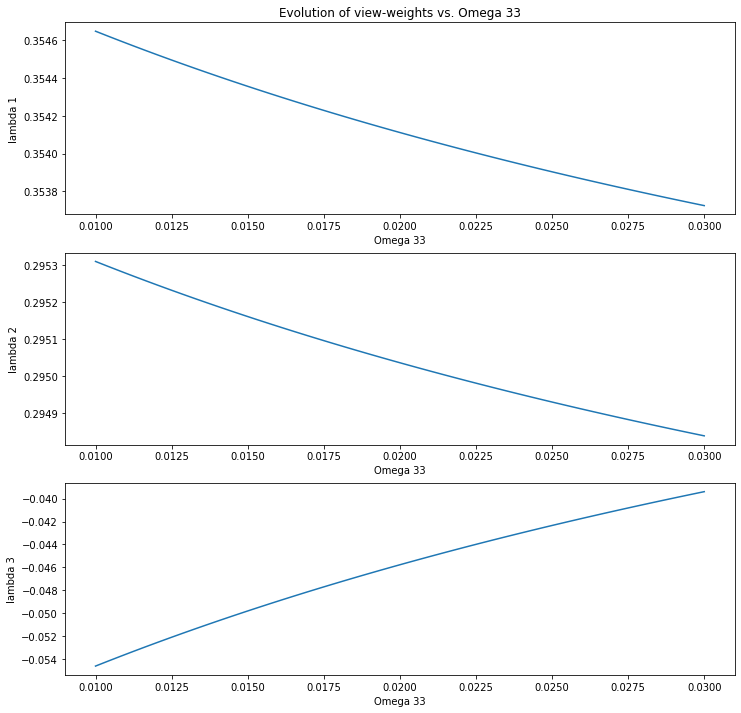
\includegraphics[scale=0.5]{ex2_1.png}
          \caption{Evolution of view-weights $\lambda_1, \lambda_2, \lambda_3$ vs. $\Omega_{33}$}
          \label{fig:fig1}
\end{figure}

\end{document}



\appendix


